We have already seen that our RL agents are able to learn near-optimal discrimination strategies and --- most importantly --- exploit them in real time, by employing exclusively the detectors' outcomes and the rewards enjoyed by the end of each episode. In this section we show that such results do not sensibly change in the presence of noise, \textit{i.e.}, that the same $Q$-learning agents are able to attain near-optimal performances even when unknown errors affect the experiment and hence the learning process. Here, we will consider dark counts, phase flip errors and the presence of a compound lossy channel acting between sender and receiver.

\textit{Dark counts}. First, we consider a common experimental imperfection known as dark counts: due to the presence of background noise, each photodetector of the receiver has a non-zero probability $p_{\rm dc}$ of detecting a photon even when it receives a vacuum signal. Accordingly, the conditional probability of obtaining an outcome $0$ given an input state $\ket\alpha$, Eq.~\eqref{eq:313singLayProb}, is modified by a multiplicative factor $(1-p_{\rm dc})$.
In Fig.~\ref{fig:dkresu} we plot $\Rt$ and $\Pt$ at time $t=5\cdot10^{5}$ for several RL strategies as a function of $p_{\rm dc}\in[0,1]$, along with the maximum success probability attainable by the corresponding receiver. We see that the final values of $\Pt$ are near-optimal for all values of $p_{\rm dc}$, while $\Rt$ seems to be slightly affected in an intermediate region of values of $p{\rm _{dc}}$. Since the agents operate on a completely model-free basis and the reward system has been chosen to ensure convergence of the value function to the true success probability, it can be expected that they are still be able to learn in the long term, as shown by the high values of $\Pt$ attained. However, since a dark count effectively increases the chance of (not) obtaining a reward for a (correct) wrong action, the time it takes to learn a near-optimal strategy and to start exploiting it might increase, as shown by the behaviour of $\Rt$.
Note that for $p_{dc}\sim 1$ the best guess is the random one and thus easier to learn.

\begin{figure}[t!]
    \centering
    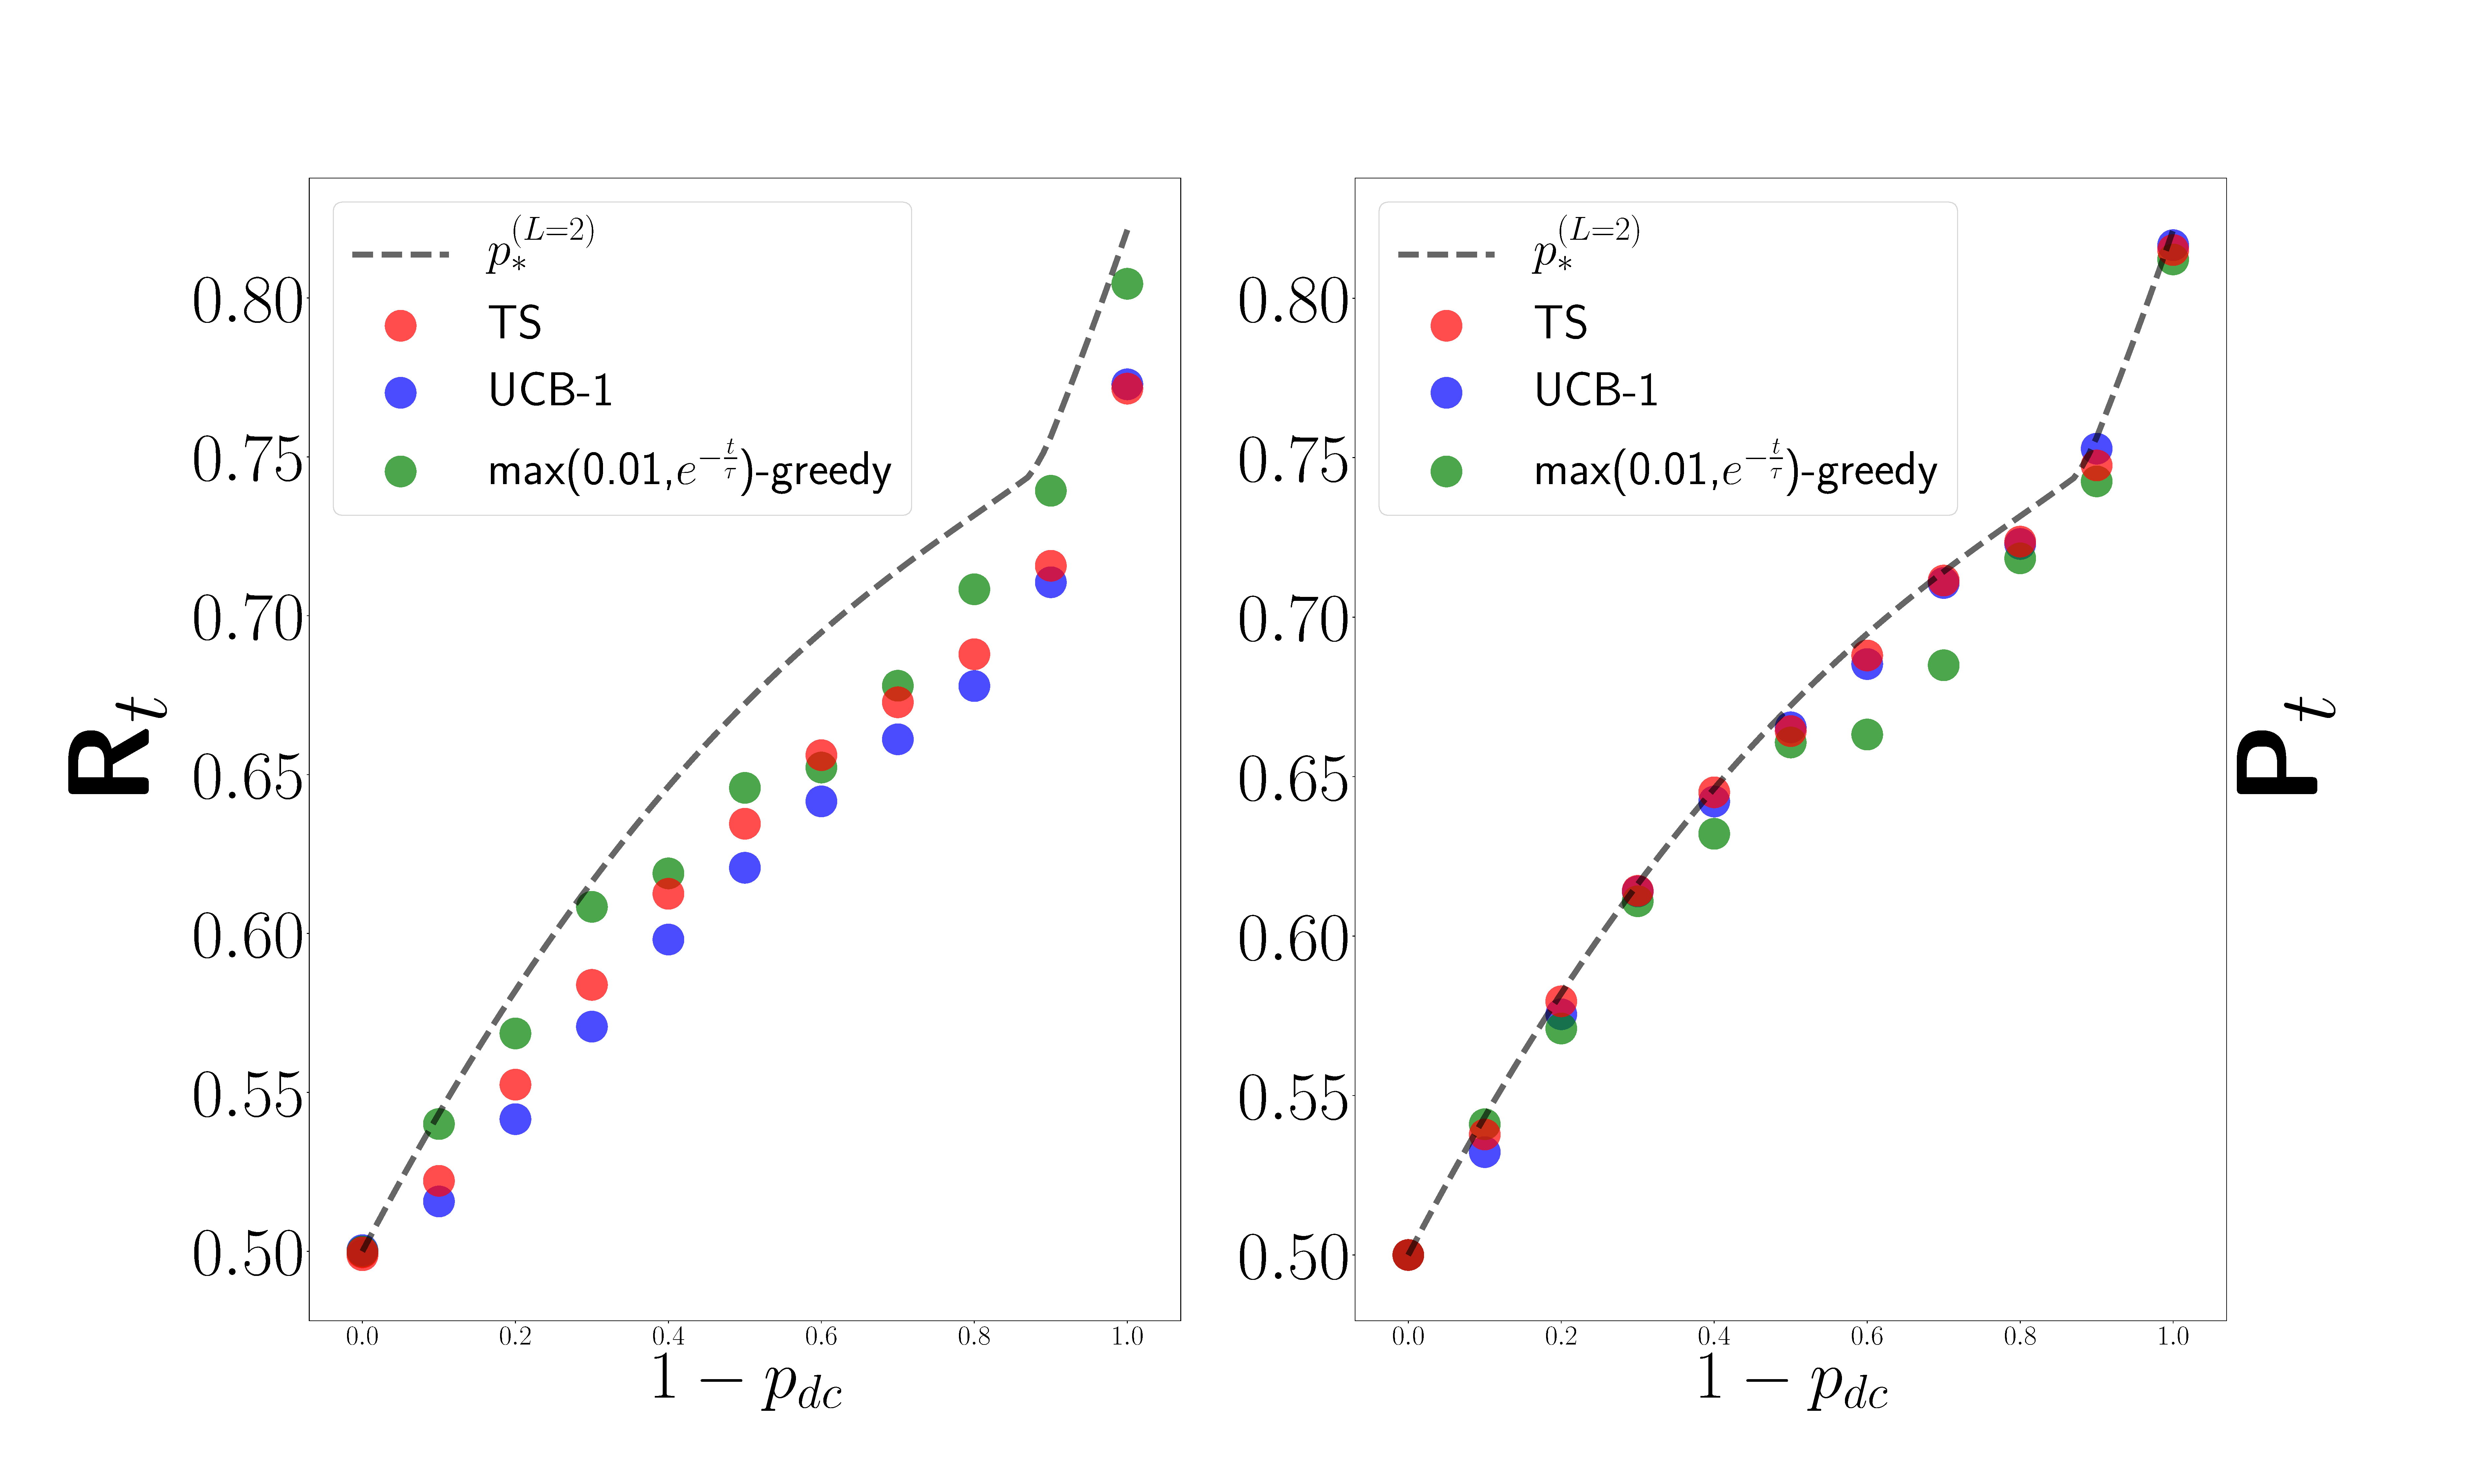
\includegraphics[width=1.\textwidth]{Figures/318/darkcounts.pdf}
   \caption{We compare the performance of the three RL agents (the same considered in Sec.~\ref{ssec:rlcoh_dolinar_plus_bandit}) at episode $t= 5\cdot 10^{5}$, for several photo-detection noise values (dark count rates). The amplitude of the coherent states is fixed to $\alpha = 0.4$; all data points are averaged over 48 agents. }
    \label{fig:dkresu}
\end{figure}

\textit{Phase flips}. Next, we consider the case where the phase of the incoming signal is flipped before arriving to the receiver, with probability $p_{f}$. In this scenario, if the agent guesses for the correct received phase, the corresponding reward will be zero since the phase initially sent was opposite than the received one. In particular, the probability of observing a string of outcomes $p(o_{1:L}|\alpha,\{a(h_{L-1})\})$ in Eq.~\eqref{eq:313singLayProb} is modified such that
\begin{align}
p(o_{1:L}|\alpha,\{a(h_{L-1})\}) &\rightarrow (1-p_f) p(o_{1:L}|\alpha,\{a(h_{L-1})\}) \\
&+ p_f p(o_{1:L}|-\alpha,\{a(h_{L-1})\})
\end{align}
In Fig.~\ref{fig:dfResults} we despict the values of $\Rt$ and $\Pt$ attained by several agents at episode $t=5\cdot10^{5}$, as a function of $p_{f}\in[0.5,1]$, along with the maximum success probability attainable by the corresponding receiver. As in the dark counts case, we see that for all values of $p_{f}$, the agents are able to converge to near-optimal $\Pt$ values and they exhibit very small variations in $\Rt$ as $p_{f}$ increases.

\begin{figure}[t!]
    \centering
    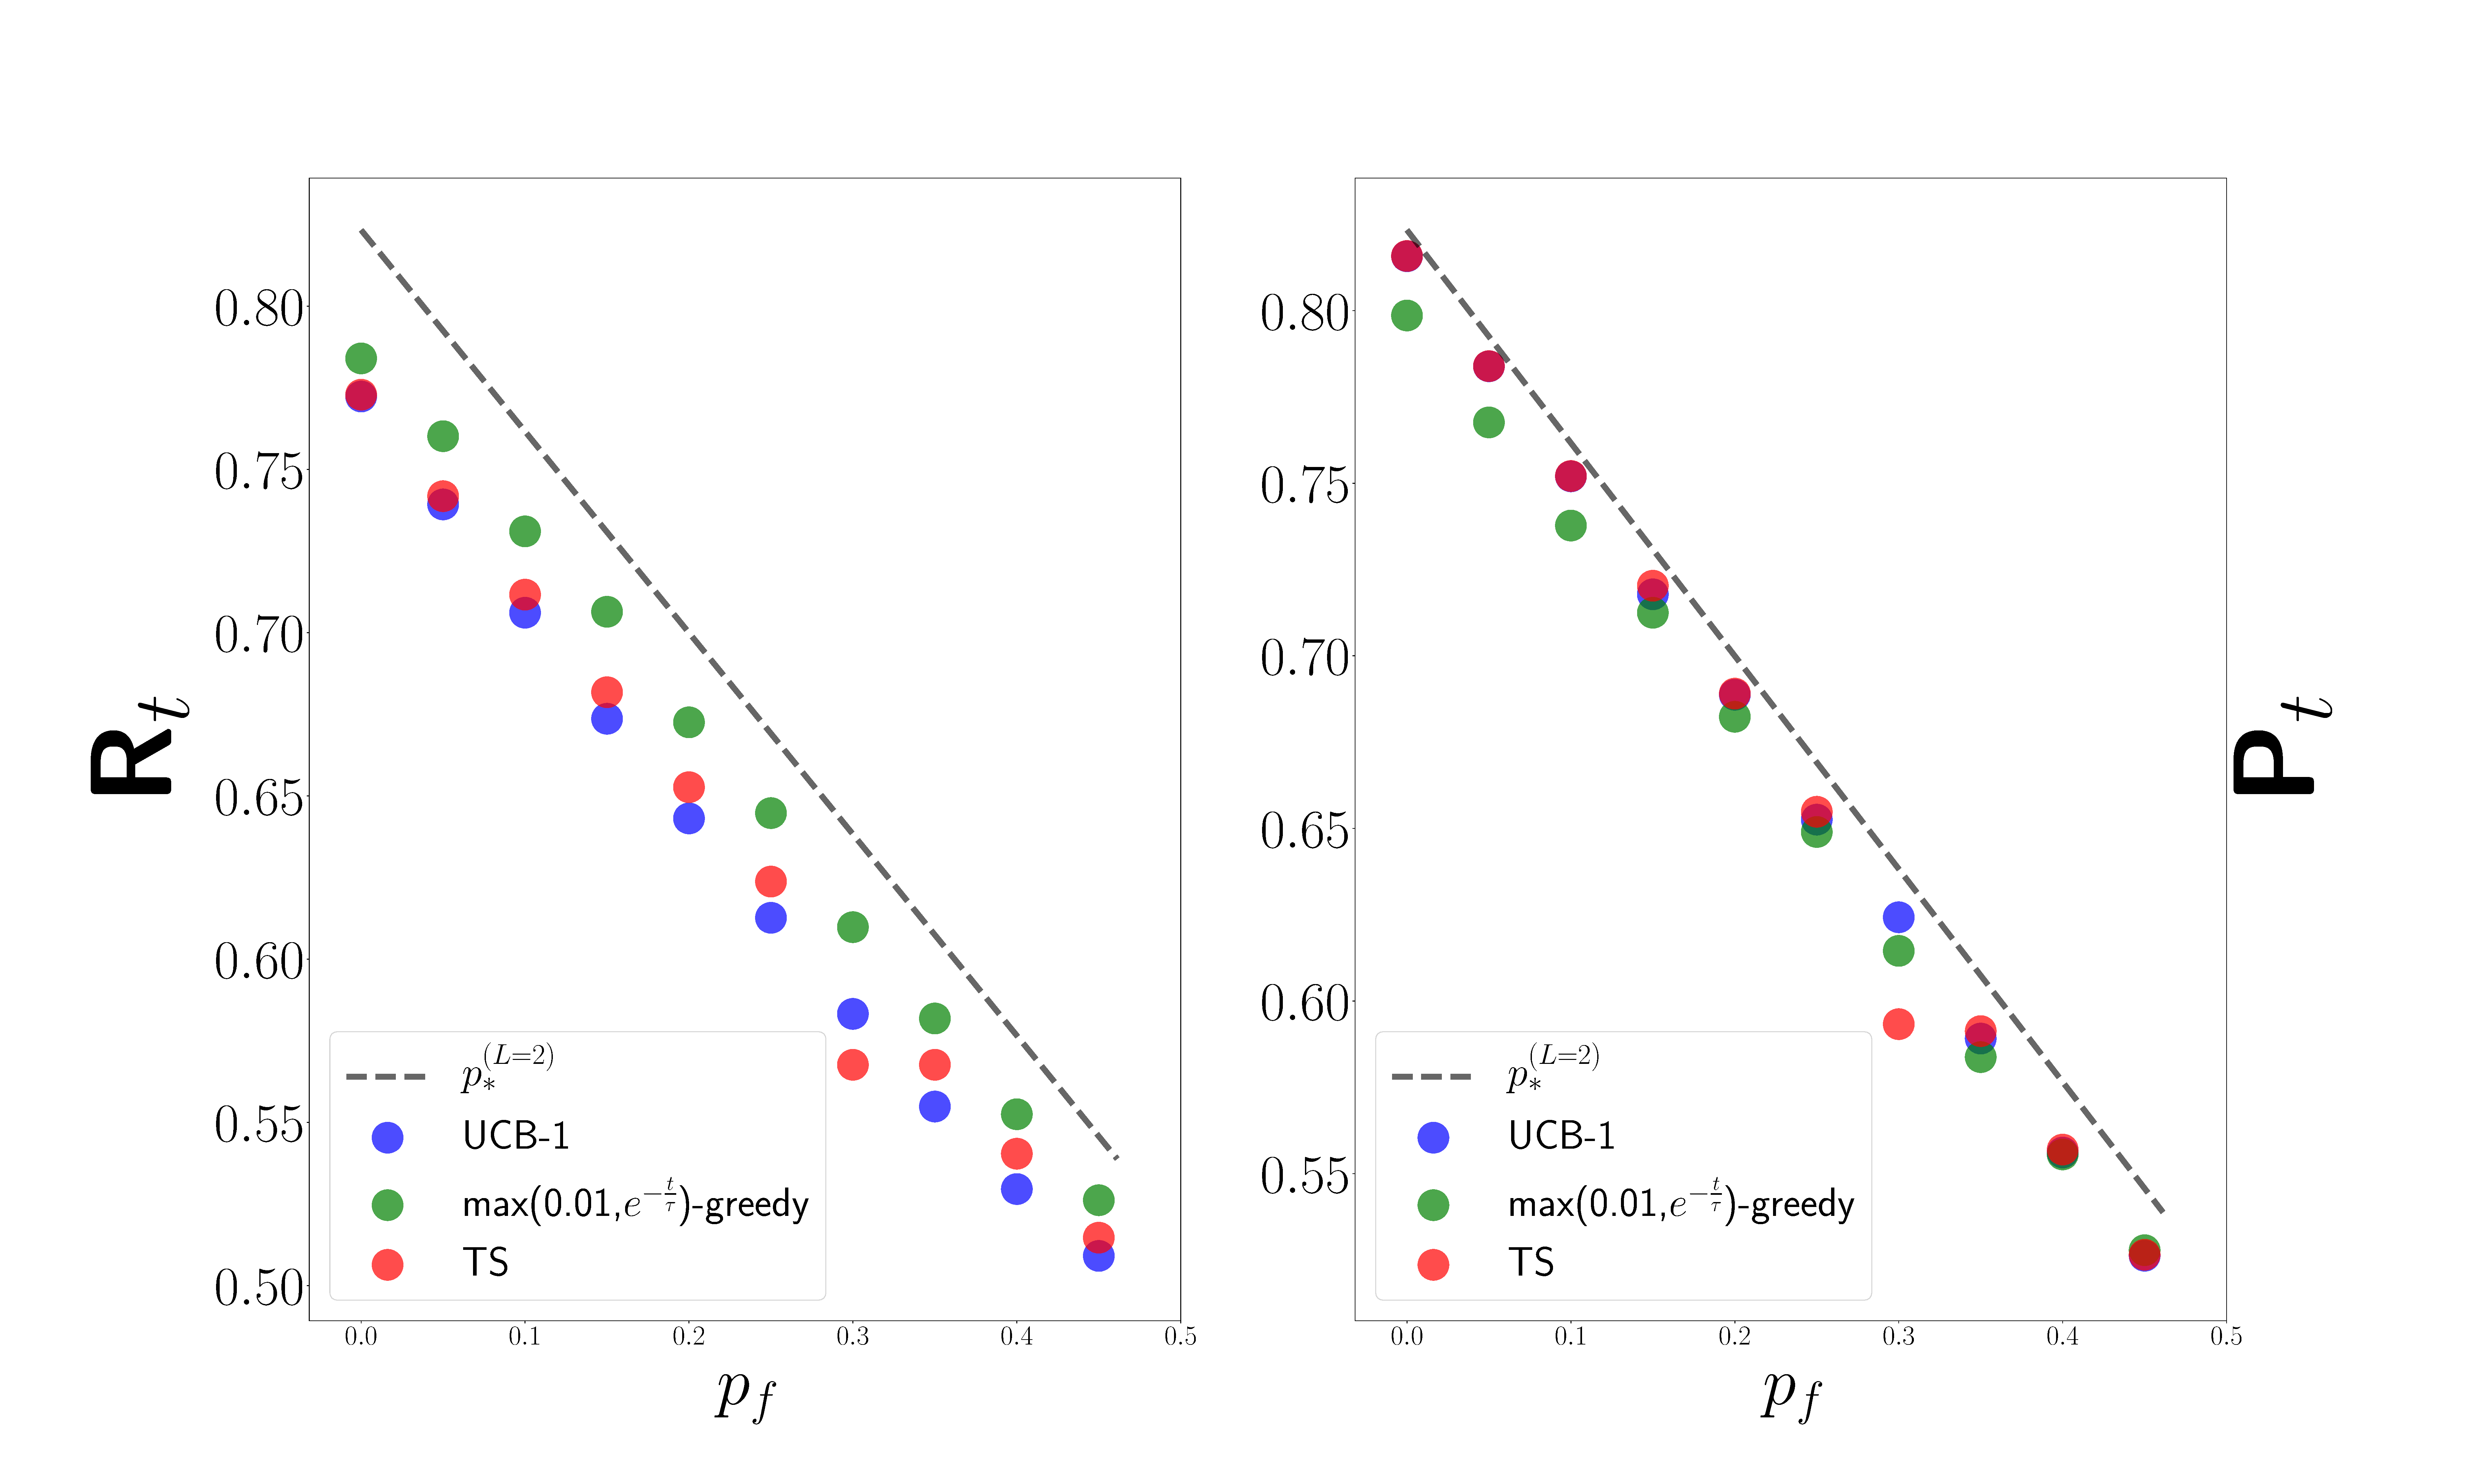
\includegraphics[width=1.\textwidth]{Figures/318/flips.pdf}
   \caption{We compare the performance of the three RL agents (the same considered in Sec.~\ref{ssec:rlcoh_dolinar_plus_bandit}) at episode $t= 5\cdot 10^{5}$, as a probability of the signal being phase flipped before arriving to the receiver. The amplitude of the coherent states is fixed to $\alpha = 0.4$; all data points are averaged over 24 agents.}
    \label{fig:dfResults}
\end{figure}

\subsubsection{Compound lossy channels}

Next, we consider the presence of lossy-channels, which are based in Ref.~\cite{bilkisitw}. These channels were introduced in Sec.~\ref{ssec:1_cv_channels}, and consist on mixing the incoming state with the vacuum state $\ket{0}$ by a beam-splitter. As such, lossy channels constitute a common model for long-distance optical-fiber and free/deep-space optical communication~\cite{Dequal2020,Andrews2005,Usenko2012a,Pirandola2021,Pirandola2021a,Vasylyev2011,Vasylyev2017}, since they model attenuations of the incoming signal; their action on coherent states reads
\begin{equation}
{\cal L}_\eta:\ket \alpha\mapsto \ket{\sqrt\eta \alpha},
\end{equation}
where $\eta\in[0,1]$ is the transmissivity or attenuation coefficient of the lossy channel.

\begin{figure}[t!]
    \centering
    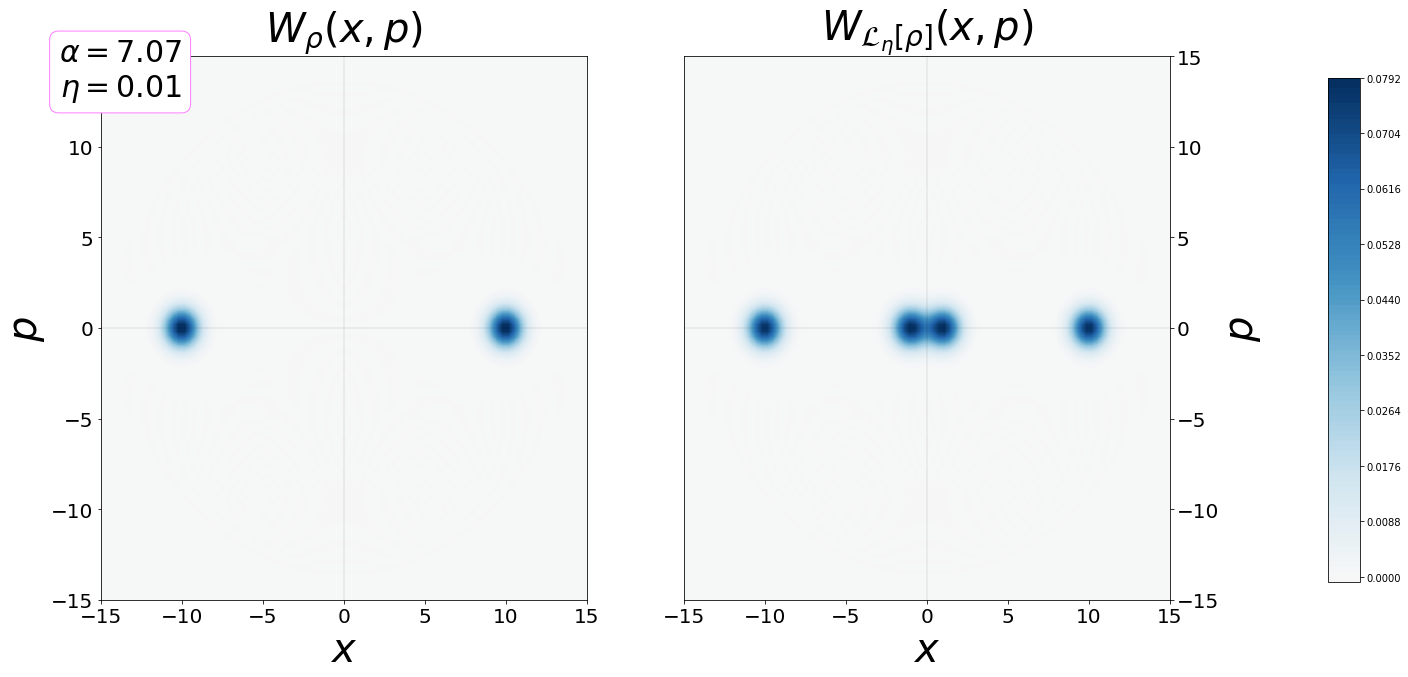
\includegraphics[width=1.\textwidth]{Figures/318/dist1wigner.png}
    \caption{We show Wigner function of inputs and outputs states of the compound channel. We observe that each input state is splitted accoriding to the possible attenuation value.}
    \label{fig:wignercomp}
\end{figure}

While we have seen that RL is effective in calibrating the receiver at different values of the noise-parameters, a considerably more challenging situation arises when practical communication links are affected by noise-parameter variations. In turn, these situation occurs in practice, and can be difficult to estimate and counteract in real-time. In particular, in the case of a lossy channel ${\cal L}_\eta$, the transmissivity $\eta$ can be altered over time, a phenomenon known as \textit{fading}, and which is caused by a plethora of different effects that alter the optical signal during its transmission through the atmosphere to/from a satellite~\cite{Dequal2020,Andrews2005,Usenko2012a,Pirandola2021,Pirandola2021a,Vasylyev2011,Vasylyev2017}. In this setting, the performance of all the receivers studied in this Chapter can be expected to degrade.

Here, we model such variable-loss channels by restricting to the case of two lossy channels $\{{\cal L}_{\eta_0}, {\cal L}_{\eta_1}\}$, happening with probabilities $\{\pi_0=\pi$, $\pi_1=1-\pi\}$, and hence the success probability%(\textit{e.g.} in Eq.~\ref{eq:1_qdisc_PSEMM})
is is now averaged over the possible channel realizations,
\begin{equation}\label{eq:meanps}
    \bar P_{\rm s}({\cal M}):=\sum_{i=0,1}\pi_i  P_{\rm s}({\cal M};\eta_i).
\end{equation}
As a consequence, the Helstrom bound will also be affected, and we will now discuss how to compute it in this case. Each hypothesis state $\ket{\alpha_k}$ can take two different values, depending on the channel transmissivity. This effectively amounts to discriminate between the two mixed states
\begin{equation}
\rho_{x}:=\sum_{i=0,1}\pi_{i}\proj{\sqrt{\eta_{i}}\alpha_{k}}, \;\;\;k\in\{0,1 \} .
\end{equation}
The average success probability of a generic measurement then reads
\begin{equation}\label{eq:pscom}
\bar P_{\rm s}({\cal M})=\sum_{k=0,1}p_{k}\tr{M_{k}\rho_{k}}
\end{equation}
and in order to compute Eq.~\ref{eq:1_qdisc_helstom}, we need to compute the trace-norm of the matrix $q_0\rho_0-q_1\rho_1$ in the four-dimensional subspace where it is supported, ${\cal S}:={\rm span}\{\ket{\psi_{k+2i}}:=\ket{\sqrt{\eta_{i}}\alpha_{k}}\}_{i,k=0,1}$. Since the trace-norm is basis-independent, one can readily find a four-dimensional representation of the involved states by computing the square-root of their Gram matrix, $B=\sqrt{G}$ with $G_{ij}=\braket{\psi_i}{\psi_j}$.
By construction it holds that $B^\dagger B= G$, hence the column vectors of $B$ constitute a representation of the original states in a $4$-dimensional subspace of the Hilbert space. By expressing all the operators via this representation, we are then able to compute the Helstrom bound in Eq.~\eqref{eq:1_qdisc_helstom} numerically.

Furthermore, we can readily compute how the homodyne success probability in Eq.~\ref{eq:gaussian_receiver_homo} is affected by this channel,
 \begin{equation}\label{eq:homodynecompo}
  P_{\rm s}^{\rm hom}=\frac{1}{2} \big( 1 + \sum_{i=0,1}\pi_{i}{\rm Erf}\left[{\sqrt{2\eta_{i}} a }\right]\big).
 \end{equation}

Finally, in the case of Dolinar-like receivers, we need to take into account that the outcome probability should now be averaged out considering the two different transmissivities:
\begin{equation}
p(j|\rho^{(\ell)}_{k}):=\sum_{i=0,1}\pi_{i}p(j|\sqrt{\eta_{i}}\alpha^{(\ell)}_{k}).
\end{equation}

Thus, we are now in position to compare the success probabilities attained by the different receivers we have studied. We note that in the case of variable-loss channels, there is no guarantee that Dolinar-like receivers will be able to attain the Helstrom bound, and whether that holds or not is an open question.

In particular, we consider the parameter regime where the two transmissivities are relatively distant from each other, which approximates the physical cases where the channel transmissivity changes abruptly due to weather conditions~\cite{Vasylyev2017}. In Fig.~\ref{fig:benchmark} we compare the behaviour of optimized Kennedy, 2-Dolinar and homodyne receivers across different values of input signal amplitude, together with the Helstrom bound. Displacements in the adaptive receivers have been numerically optimized using simulated annealing~\cite{dual_annealing, scipy}. This optimization proves demanding for higher number of adaptive measurements, and thus the dynamic programming method presented in Sec.~\ref{sec:rlcoh_model_aware_approach_intro} fails, unless a sufficiently high amount of computational resources is allocated to perform the continuous optimization (for instance, several initializations per optimization seed, and several seeds), though we have not investigated this optimization further.

\begin{figure}[t!]
   \centering
   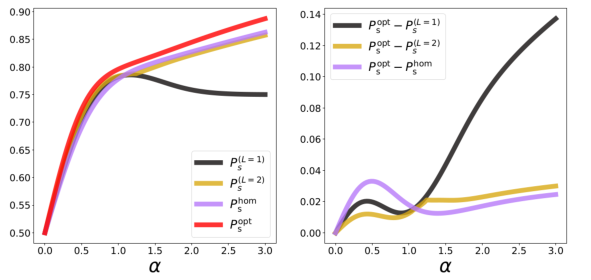
\includegraphics[width=1.\textwidth]{Figures/318/singleetas[0.01, 1]_wdiffe_.pdf}
   \caption{Top: We compare the success probabilities attainable by one $(L=1)$ and two ($L=2$) adaptive receivers with homodyne measurement and Helstrom bound, for different values of signal intensity. Bottom: difference between the success probabilities of the receivers under considerations and the Helstrom bound are shown in order to ease the visualizaton of different features. In this case, a lossy channel ($\eta=10^{-2}$) acts on the transmitted state with probability of one half, whereas the signal is transmitted through a noise-less channel otherwise. }
   \label{fig:benchmark}
\end{figure}

We observe that, while the homodyne receiver maintains a satisfying performance in the whole amplitude range, the behaviour of the Kennedy receiver exhibits a clear transition and its performance degrades at sufficiently large amplitudes. Fortuantely, the addition of a second adaptive detection layer appears to be able to correct this trend. Hence the two-layer receiver can get close to the performance of the homodyne receiver in the large-amplitude regime, while showing a clear advantage with respect to the latter in the low-amplitude regime.

The degrade of $1$-Dolinar receivers in the high-amplitude regime can be understood as follows. The action of the compound channel, for high-amplitude signals, is that of increasing the possible candidates in the discrimination problem to four; each channel can act with probability $\frac{1}{2}$, and while the success probability in Eq.~\ref{eq:pscom} weights only the final binary guess, the action of the compound channel is that of averaging out two binary discrimination problems: the original one (with states $\ket{\pm \alpha}$), and the new one (with states $\ket{\pm \eta \alpha}$). In this sense, if initial amplitudes are small, then the attenuated amplitude will be \textit{very} small, and the resulting state will effectively be the vacuum state.

One can understand this results by looking at the phase space in Fig~\ref{fig:wignercomp}. The kennedy reciver efectivly projects over $\proj{\beta}$. Therefore it checks whether the hypothesis occupies a small region around $\beta$ or not. In the case of composite hypothesis the coherent state projection can only cover one of the states in the ensemble. This effect is reduced when the amplitude is very low, and the \textit{blobs} for both coherent states can be partially covered by the coherent state projection. In the limit of very large amplitudes, where the signals are almost orthogonal, a Kennedy receiver will need to specialize on one of the members of the ensemble, which will lead to a succes probability of $\frac{3}{4}$, instead of 1.

On the contrary, a $L$-Dolinar receiver performs a projection on a coherent state $\ket{\beta_\ell}$ (v. the rest), at each $\ell$. Thus, such receiver is expected to attain a probability 1 for large amplitudes, if the number of hypothesis ---composite or not--- can be covered by $L$ coherent states.

Finally, in Fig.~\ref{fig:epgreedycomp} we show that our Q-learning agent is also capable of calibrating a $2$-Dolinar receiver under the composite noisy channel, without prior informaton about the original amplitudes nor the attenuations.

 \begin{figure}[t!]
     \centering
     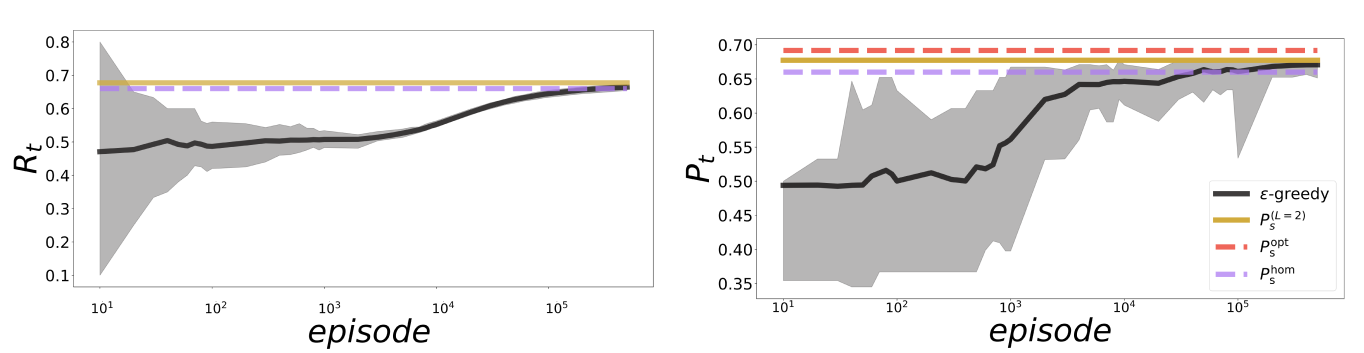
\includegraphics[width=1.\textwidth]{Figures/318/compoundRL.png}
     \caption{We show learning curve behaviour for $\epsilon$-greedy Q-learning, with an $\epsilon$ exponentially decaying as a function of episode number. The figures of merit are averaged over $48$ agents and corresponding uncertainty region are shown.}
     \label{fig:epgreedycomp}
 \end{figure}

To sum up, our numerical simulations indicate that model-free $Q$-learning agents can readily adapt to many situations that are present in experimental scenarios. As a matter of fact, we have considered dark counts, phase flips and lossy channels with varying transmissivity. 
%%
